% !TeX root = ./LetsDriveDipl.tex
\def \currentAuthor {Nicolas Frey} %so kann jederzeit der Autor geändert werden -> wird in der Fusszeile angezeigt.

\chapter*{Einleitende Bemerkungen}



\chapter*{Notationen}
Beschreibung wie Code, Hinweise, Zitate etc. formatiert werden  



\chapter{Einleitung}



\chapter{Projektmanagement}



\section{Metainformationen}
Dieses Kapitel dient der Vorstellung der Schlüsselpersonen und Kooperationspartner, die an der Entstehung dieser Diplomarbeit beteiligt sind. Hier werden das Forschungsteam, die Betreuerin, der Partner und der Ansprechpartner kurz vorgestellt. Die Zusammenarbeit dieser Akteure ist von zentraler Bedeutung für den Erfolg und die Qualität dieser Arbeit.

\subsubsection*{Team}

\emph{Nicolas Frey} \\
\href{mailto:nfrey@tsn.at}{nfrey@tsn.at} 
\begin{figure}
	% include gfx Nicolas Frey Bild
\end{figure}

\emph{Matthias Leiter} \\
\href{mailto:mattleiter@tsn.at}{mattleiter@tsn.at} 
\begin{figure}
	% include gfx Matthias Leiter Bild
\end{figure}

\emph{Anja Holzknecht} \\
\href{mailto:anjholzknecht@tsn.at}{anjholzknecht@tsn.at} 
\begin{figure}
	% include gfx Anja Holzknecht Bild
\end{figure}

\subsubsection{Betreuer}
\emph{Melanie Osl}

\subsubsection{Partner}
\textbf{icotec Graz} \\
\href{mailto:office@icotec.at}{office@icotec.at} \\
\href{www.icotec.at}{www.icotec.at} \\
Andritzer Reichsstraße 15 \\
8045 Graz \\
Tel.: \href{tel:069910624227}{0699 10624227}
% TODO : qualität von logo
\begin{figure}[H]
	\captionsetup{singlelinecheck = false, format= hang, justification=raggedright, font=footnotesize, labelsep=space}
	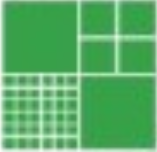
\includegraphics{figures/Logo_Projektpartner.png}
	\caption{Logo der Firma icotec}
	\label{fig:LogoProjektpartner}
\end{figure}

\subsubsection{Ansprechpartner}
\emph {Ronald Macek}
\begin{figure}
	% include gfx Ronald Macek Bild
\end{figure}


\section{Vorerhebungen}
In den Vorerhebungen werden der IST - Zustand und der SOLL - Zustand genau erklärt. Eine Zielformulierung beschreibt das erwartete Ergebnis eindeutig, attraktiv, realistisch und messbar mit konkreten Terminen. Einfluss, Nähe und Einstellung der Stakeholder und Maßnahmen für diese werden graphisch und tabellarisch dargestellt.

\subsection{IST-Zustand}
Bis dato gibt es keine App, die das Aufzeichnen des Fahrtenbuchs für den Führerschein mit L-Tafel unabhängig von Fahrschulen und Mitgliedschaften (ÖAMTC) ermöglicht. Des Weiteren gibt es kein weitverbreitetes Tool das dem/der Fahrschüler:in personalisiertes Feedback seines/r bisherigen Fahrten bekommt.

\subsection{SOLL-Zustand}
Eine Smartphone-App für Fahrschüler:innen, welche über GPS - Tracking automatisch Einträge in einem Fahrtenbuch erstellt. Diese Einträge werden in Form eines offiziellen Protokolls exportiert. Das Analysieren der Fahrdaten und Erzeugen von Statistiken geben dem/der Fahrschüler:in ein Feedback. Zur Datensicherung steht eine Datenbank zur Verfügung.

\subsection{Projektzieleplan}
Ziel ist die Erstellung einer Smartphone-App für Fahrschüler:innen, welche über GPS - Tracking automatisch Einträge in einem Fahrtenbuch aufzeichnet. Diese Einträge sollen in Form eines offiziellen Protokolls an die Fahrschule ausgehändigt werden können. Um Schüler:innen besser auf die praktische Fahrprüfung vorzubereiten, soll ebenso ein digitaler Fahrlehrer implementiert werden, dem/der Schüler:in Feedback in Form von statistischen Auswertungen gibt. Bis zum 28.6.2024 sollen alle oben genannten Features implementiert, getestet und veröffentlicht werden. Um sich ein Bild vom Markterfolg machen zu können, werden hierbei die App-Store Bewertungen und Downloadzahlen verwendet. Das Ziel ist, bis September die 3\%-Schwelle zu erreichen, das bedeutet etwa 100 Neukunden unter allen Österreicher:innen, die die L-Tafel beantragen (einschließlich L-17).

\subsection{Projektumfeldanalyse}

\subsubsection*{Identifikation der Stakeholder}
Zu Beginn haben wir mittels „Brainstorming“ die wichtigsten Stakeholder identifiziert. Uns wurde ersichtlich, dass nur User also Fahrschüler:innen und Begleitpersonen unsere Zielgruppen sind und mit dem Produkt zufrieden sein müssen. Im Laufe der Recherche wurde eine von ÖAMTC bereitgestellte\hfill\break Konkurrenz-App identifiziert, wodurch uns sofort klar war, dass wir gleich von Beginn an ein starkes Auftreten brauchen. Das bedeutet, dass wir speziell durch bessere Software und Features, sowie durch ein besseres Preismodell attraktiver für den Kunden sein wollen. Die Stakeholder werden mithilfe der folgenden Tabellen und Abbildungen (\cref{tab:Charakterisierung}, \cref{tab:Maßnahmen}, \cref{fig:Stakeholder}) dargestellt.



\subsubsection*{Charakterisierung der Stakeholder}
\begin{table}[H]
	\centering
	\begin{tabularx}{\textwidth}{|l|l|l|l|X|}
		\hline
		\textbf{Stakeholder} & \textbf{Einfluss} & \textbf{Nähe} & \textbf{Einstellung} & \textbf{Beschreibung} \\
		\hline
		Auftraggeber & groß & nahe & positiv & Geschäftsführer \\
		\hline
		Fahrschulen & groß & mittel & neutral & Die Fahrschulen, welche die Fahrschüler:innen ausbilden. \\
		\hline
		Begleitperson & groß & nahe & positiv & z.B Eltern der Fahrschüler:innen \\
		\hline
		Fahrschüler:innen & groß & nahe & positiv & Die Fahrschüler:innen selbst \\
		\hline
		Medien & gering & mittel & neutral & Alle Medien die Über diese App berichten. \\
		\hline
		Konkurrenz-Apps & groß & nahe & negativ & Konkurrenz-Apps z. Bsp.: ÖAMTC \\
		\hline
	\end{tabularx}
	\caption{Charakterisierung der Stakeholder}
	\label{tab:Charakterisierung}

\end{table}

\subsubsection*{Maßnahmen}
\begin{table}[H]
	\centering
	\begin{tabularx}{\textwidth}{|l|X|}
		\hline
		\textbf{Stakeholder} & \textbf{Maßnahmen} \\
		\hline
		Auftraggeber & Wöchentliche Meetings. Berichte und Fortschritte liefern. \\
		\hline
		Fahrschulen & Überzeugen, dass das Protokoll weniger leicht verfälscht werden kann und die App die Fahrschüler:innen unterstützt. \\
		\hline
		Begleitperson & Protokollierung mittels App soll eine Erleichterung sein und Schutz vor Datenverlust bieten. \\
		\hline
		Fahrschüler:innen & Positive Werbung, benutzerfreundliches und praktisches Design der App, sowie werbungsfrei. \\
		\hline
		Medien & Durch Erfolg und hohe Userzahlen, sowie gutes Marketing / auf App aufmerksam machen. \\
		\hline
		Konkurrenz-Apps & Faires Konkurrenzverhalten \\
		\hline
	\end{tabularx}
	\caption{Maßnahmenkatalog}
	\label{tab:Maßnahmen}
\end{table}


\subsubsection*{Grafische Darstellung des Umfeldes}
\begin{figure}[H]
	\centering
	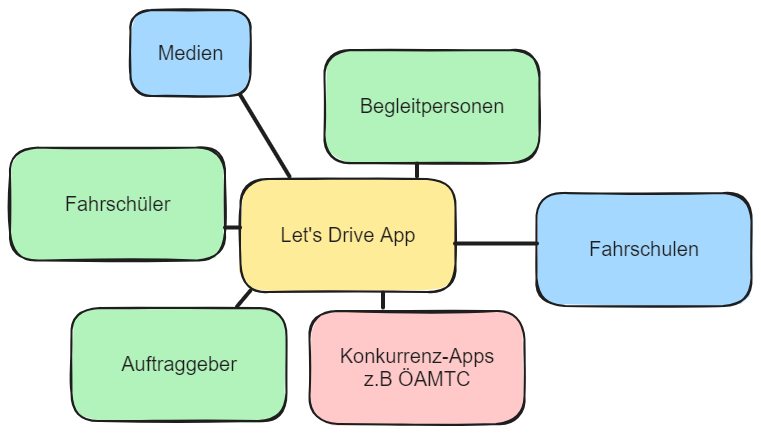
\includegraphics[width=15cm]{figures/graf_stakeholder.png}
	\caption{Grafik Stakeholder}
	\label{fig:Stakeholder}
\end{figure}


\subsection{Risikoanalyse}
Die Entwicklung digitaler Anwendungen, insbesondere mobiler Apps, geht mit vielfältigen Risiken einher, die Sicherheit und Funktionalität beeinträchtigen können. Aber auch externe Einflüsse können ein Projekt gefährden. Um für den Ernstfall gerüstet zu sein wird daher eine Risikoanalyse von Let's Drive App gemacht. Es gilt potenzielle Gefahren zu identifizieren, zu bewerten und geeignete Maßnahmen zur Risikominderung zu erarbeiten. Diese werden mittels einer Risikomatrix (Abbildung \ref{fig:Risikomatrix}) und Tabellen (Identifizierung der Risiken in Tabelle \ref{tab:Identifizierung}, und Einstufung der Risiken in Tabelle \ref{tab:Risikoeinstufung} \& \ref{tab:Legende}) erörtert und beschrieben.


\begin{minipage}{\textwidth}
	Diese Kategorien werden für die Tabelle verwendet:
	\begin{itemize}[itemsep=0pt,parsep=0pt]
		\item \textbf{W} wirtschaftlich
		\item \textbf{P} produktbezogen
		\item \textbf{M} menschlich
		\item \textbf{R} rechtlich
		\item \textbf{T} technisch
	\end{itemize}
\end{minipage}

		In Tabelle \ref{tab:Identifizierung} werden als erstes alle Risiken benannt und einer Kategorie zugeordnet. Anschließend wird versucht die Folgen und Maßnahmen, soweit man das voraussagen kann, zu beschreiben.

\begin{table}[H]
	\centering
	\begin{tabularx}{\textwidth}{|p{5cm}|p{2cm}|p{2cm}|X|}
		\hline
		\textbf{Risiko} & \textbf{Kategorie} & \textbf{Folgen} & \textbf{Maßnahmen} \\
		\hline
		Konkurrenz hat besseres Produkt & W, T & weniger User & vorhandene Features verbessern, neue Features hinzufügen \\
		\hline
		App wird nicht gut angenommen & P, W & weniger User & mehr Marketing \\
		\hline
		Tracking für Schüler wird nicht erlaubt & R & Feature fällt weg & Begleitperson übernimmt dieses Feature vollständig \\
		\hline
		App ist wirtschaftlich uninteressant & W & geringe Einnahmen & Werbung einbauen (Einnahmen sind nicht der Fokus der Projektgruppe.) \\
		\hline
		Das Deployment für alle Plattformen ist von Beginn an nicht möglich & W & Plattform fehlt zu Beginn & Da ein Apple-Computer für die Kompilierung erforderlich ist,wir dieser Teil von der Partnerfirma übernommen \\
		\hline
		Maui ist ein ganz neues Framework und nicht in jedem Bereich gleich gut, wie andere oder nativ programmierte Apps & T & weniger Support und Dokumentation & keine  \\
		\hline
	\end{tabularx}
	\caption{Identifizierung der Risiken}
	\label{tab:Identifizierung}	
\end{table}

\newpage
In Tabelle \ref{tab:Risikoeinstufung} wird nun das Risiko bewertet. Dabei ergibt die Eintrittswahrscheinlichkeit mal der Auswirkung das Risikopotenzial. Die Werte für diese Rechnung liegen dabei im Bereich von 1 bis 10 inklusive. Somit liegt das berechnete Ergebnis zwischen 0 und 100. Die Legende in Tabelle \ref{tab:Legende} erklärt die Interpretation dieses Ergebnisses ganz genau.
\begin{table}[H]
	\centering
	\begin{tabularx}{\textwidth}{|X|c|c|c|}
		\hline
		\textbf{Risiko} & \textbf{Eintrittswahrsch.} & \textbf{Auswirkung} & \textbf{Risikopotential} \\
		\hline
		Konkurrenz ist besser & 4 & 8 & 32 \\
		\hline
		App wird nicht gut angenommen & 5 & 8 & 40 \\
		\hline
		Tracking für Schüler wird nicht erlaubt & 2 & 6 & 12 \\
		\hline
		App ist wirtschaftlich uninteressant & 8 & 2 & 16 \\
		\hline
		Das Deployment für alle Plattformen ist von beginn an nicht möglich & 4 & 4 & 16 \\
		\hline
		Maui ist ein neues Framework und ist nicht in jedem Bereich gleich gut wie andere oder native programmierte Apps & 5 & 5 & 25  \\
		\hline
 	\end{tabularx}
	\caption{Risikoeinstufung}
	\label{tab:Risikoeinstufung}	
\end{table}

\begin{table}[H]
	\centering
	\begin{tabular}{|c|c|c|r|}
		\hline
		\textbf {} & \textbf{Wahrscheinlichkeit} & \textbf{Auswirkung} & \textbf{Wahrscheinlichkeit x Auswirkung} \\
		\hline
		1 & gering 		& gering 		& W x A \quad < 20.....\\
		\hline
		2 & mittel 		& mittel 		& W x A \quad = 21-40\\
		\hline
		3 & hoch   		& hoch 			& W x A \quad = 41-60\\
		\hline
		4 & hoch 	& sehr hoch			& W x A \quad = 61-80\\
		\hline
		5 & sehr hoch 	& katastrophal		& W x A \quad  > 81.....\\
		\hline
	\end{tabular}
	\caption{Legende zur Risikoeinstufung}
	\label{tab:Legende}
\end{table}

\newpage
Die Risikomatrix stellt nun die in Tabelle \ref{tab:Risikoeinstufung} berechneten Werte grafisch dar. Dabei ist die Risikoakzeptanzlinie eine entscheidende Trennung zwischen Risiken mit dem man leben kann und Risiken die ein ernstes Problem sein können.
\begin{figure}[H]
	\centering
	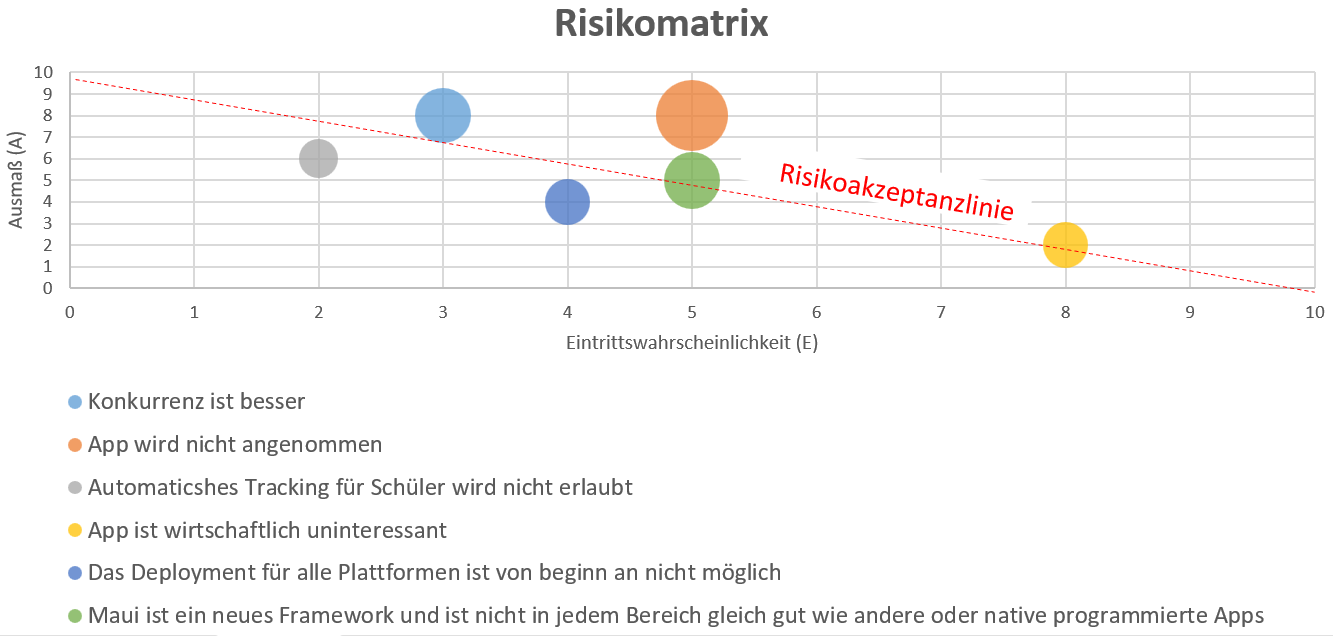
\includegraphics[width=15cm]{figures/Risikomatrix.png} %TODO grafik einblenden und beschreiben
	\caption{Risiko Matrix}
	\label{fig:Risikomatrix}
\end{figure}

\newpage
\section{Pflichtenheft}

Das Pflichtenheft ist ein wichtiger Bestandteil der Erörterung der Anforderungen des Projektes. Es beinhaltet das Lastenheft und beschreibt wie diese Aufgaben umgesetzt werden und wie das Endprodukt dabei entstehen soll. Das würde eigentlich den gesamten Punkt \ref{sec:problemanalyse} miteinbeziehen in dem die Use Cases und Ablaufdiagramme beschrieben sind. Das wird aber in dieser Arbeit unter eigenen Punkten behandelt.

\subsection{Zielbestimmung}
Es muss immer ein Produkt konstruiert werden welches die Anforderungen des Kunden und nicht die der Firma erfüllt. Im Pflichtenheft werden alle Muss Anforderungen beschrieben, die an diese Software gestellt werde. Weiters werden die Kann Anforderungen beschrieben. Beides kommt vom Kunden. In den Nicht Zielen wird nochmals auf ein paar wichtige Punkte eingegangen für die diese App nicht gedacht ist. In unserem Fall sind die eigentlichen Kunden die User der App.

\subsection{IST-Zustand}
Bis dato gibt es keine App, die das Aufzeichnen des Fahrtenbuchs für den Führerschein mit L-Tafel unabhängig von Fahrschulen und Mitgliedschaften (ÖAMTC) ermöglicht. Des Weiteren gibt es kein weitverbreitetes Tool das dem/der Fahrschüler:in personalisiertes Feedback seines/r bisherigen Fahrten bekommt.

\subsection{SOLL-Zustand}
Eine Smartphone-App für Fahrschüler:innen, welche über GPS - Tracking automa-
tisch Einträge in einem Fahrtenbuch erstellt. Diese Einträge werden in Form eines
offiziellen Protokolls exportiert. Das Analysieren der Fahrdaten und Erzeugen von
Statistiken geben dem/der Fahrschüler:in ein Feedback. Zur Datensicherung steht
eine Datenbank zur Verfügung. Auch ein manuelles Hinzufügen einer Fahrt soll möglich sein.

\subsection{NICHT-Ziele}
Ziel der Projektarbeit ist es nicht eine Release-Software fertigzustellen. Ein Prototyp der funktioniert ist ausreichend. Die gesammelten Daten werden nur für persönliche Feedbacks verwendet. Es werden keine Daten weitergegeben.

\subsection{Produkteinsatz und Umgebung}

	Das Produkt wird eine Cross-Platform App, welche auf den Betriebssystemen Android und iOS erhältlich sein wird. Let's Drive findet Anwendung bei Fahrschüler:innen, welche die L-Tafel oder den L-17 Fahrschein absolvieren wollen. Dienste der App beinhalten z.B. Tracking, Statistik der Fahrten, einfacher Export der Tracking Daten in das Formular für den Fahrschein mit 3000 bzw. 1000 Kilometer. Ein GPS wird für das Tracking benötigt. Eine Internetverbindung ist während einer Fahrt nicht erfordelich.

\subsection{Funktionalitäten}

	Es gibt grundsätzlich 2 Arten von Anforderungen. Diese, die in der App sein müssen und diese, die in der App sein können. Die Muss Anforderungen müssen natürlich vollständig umgesetzt werden. Weiters gibt es die FURPS - Anforderungen. Das sind funktionale Anforderungen und die nicht für die Funktion der App notwendigen Anforderungen wie Benutzerfreundlichkeit, Zuverlässigkeit, Leistung und Support. \par
	Funktionale MUSS-Anforderungen beinhalten u.A. zuverlässiges und Fehlerfreies Tracking der Strecke, zuverlässige Datenbankaktualisierung, zuverlässiger pdf Export und manuelle Einträge unterstützen Feedback über die aufgezeichneten Fahrten geben. Nicht-Funktionale MUSS-Anforderungen sind ein ansprechendes Userinterface, eine einfache und flüssige Menüführung und Erweiterbarkeit. \par
	Funktionale KANN-Anforderungen beinhalten Prüfungsfahrten simulieren mit Audioausgabe der Strecke und Erweiterbarkeit des Einsatzbereiches mittels generalisierung der App (Führung eines generellen Fahrtenbuches). Nicht Funktionale umfassen dabei, dass verschiedene Designs gefertigt werden können und die App in mehreren Sprachen verfügbar ist.

\subsection{Testszenarien und Testfälle}

Unit Tests sind der erste Schritt, danach werden Integrationstests durchgeführt. Nach proof of concept und Abdeckung der meisten Testfälle werden eigenständige Alpha-Tests innerhalb des Entwicklungs-Teams durchgeführt. Dies beinhaltet einen Dev-Account, das Aufzeichnen von Fahrten und der Upload in die Datenbank. Danach sollen Beta-Tester (Bekannte und Freiwillige) die App testen, indem wir sie für Beta-Tester auf den App-Stores zu Verfügung stellen.
\begin{itemize}
	\item Fahrt starten und aufnehmen / Die Genauigkeit des Trackings ermitteln
	\item Fahrt in die Datenbank hochladen / auf den lokalen Speicher legen
	\item Fahrt abbrechen / während der Fahrt abbrechen
	\item Fahrt durch den Tunnel / während man kein GPS-Signal hat
	\item An- und Abmeldung bei mehreren App-Instanzen beim gleichen Account
	\item Manuelles Löschen und Anlegen von Fahrtenbuch Einträgen
\end{itemize}
\subsection{Liefervereinbarung}
Bereitstellung der App im Apple App-Store, im Google Play Store und eventuell in der Huawei App-Gallery. Damit kann die App allen österreichischen Fahrschüler:innen zur Verfügung gestellt werden.

\section{Problemanalyse}
\label{sec:problemanalyse}
In diesem Abschnitt werden mittels UML Diagrammen und Beschreibungen die Funktionalitäten beschrieben. Auch das Userinterface wird dargestellt. Eine gründliche Untersuchung dieser Funktionellen und nicht Funktionellen Anforderungen wird dazu beitragen die Wünsche der Benutzer zu definieren um die App nutzerfreundlich und nach Wunsch des Kunden zu designen. Das soll der Grundbaustein für unsere weitere App Entwicklung sein.

\subsection{USE-Case-Analyse}

USE-Cases, auch Anwendungsfälle genannt, sind eine wichtige Komponente in einer Diplomarbeit. Sie beschreiben, wie ein bestimmtes System oder eine Software in der Praxis eingesetzt wird. Auch Zusammenhänge sind ersichtlich. Dabei unterscheidet man zwischen benutzerbasierten und ereignisbasierten USE-Cases.

\begin{itemize}
	\item Ich als Begleitperson möchte die gefahrenen Routen automatisch aufgezeichnet bekommen.
	\item Ich als Begleitperson möchte eine Fahrt manuell hinzufügen können.
	\item Ich als Nutzer der App möchte eine Liste der unternommenen Fahrten haben.
	\item Ich als Begleitperson möchte die gefahrenen Routen als PDF-Dokument drucken können.
	\item Ich als Fahrschüler:in möchte durch den digitalen Fahrlehrer auf die praktische Fahrprüfung vorbereitet werden.
	\item Als Fahrlehrer:in möchte ich die Fahrdaten auswerten können.
	\item Als Benutzer dieser App möchte ich meine Daten sichern können.
	\item Ich als Fahrlehrer:in möchte Einsicht auf die gefahrenen Strecken und den Fortschritt meiner Fahrschüler:in haben.
	\item Ich als Fahrschule möchte die Validität der gefahrenen Strecken der Fahrschüler:innen sicherstellen können.
	\item Ich als Fahrschüler:in möchte, wenn es einen Netzausfall oder einen GPS-Ausfall gibt, trotzdem meine Daten absichern und eine Fahrt weiterführen können.
\end{itemize}


Das folgende UML USE-Case-Diagramm (\ref{fig:USE-Case-Diagramm}) zeigt graphisch die Userstories und wie sie in der Anwendung zusammenhängen.

\begin{figure}[H]
	\centering
	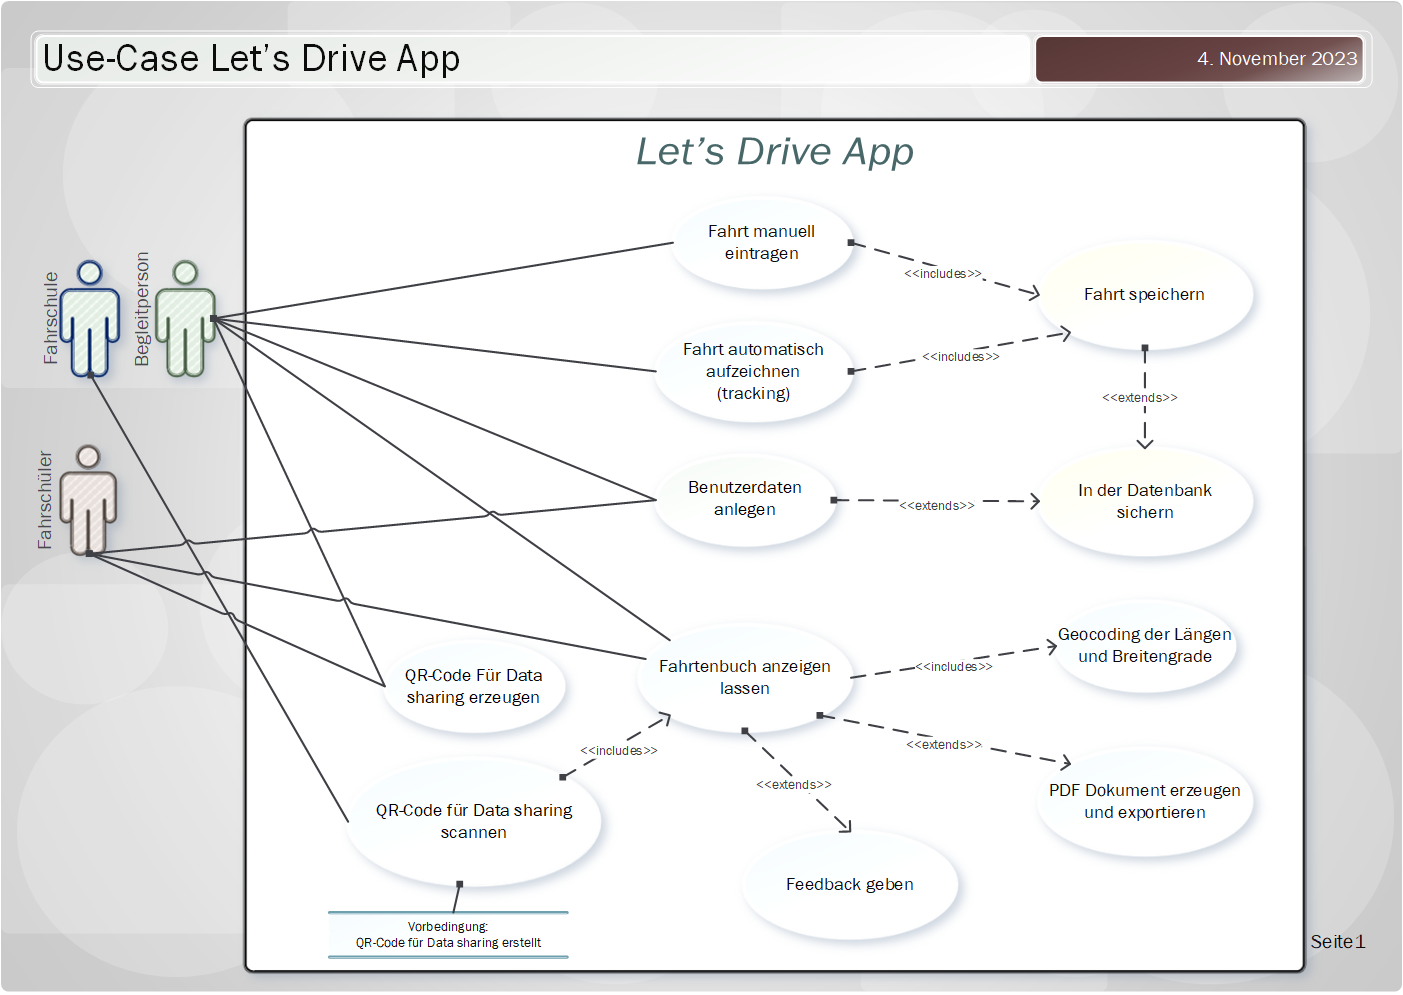
\includegraphics[width=15cm]{figures/usecase_diagramm.png}
	\caption{USE-Case Diagramm}
	\label{fig:USE-Case-Diagramm}
\end{figure}

Die nachfolgenden schriftlichen Detailbeschreibungen in Tabellen \ref{tab:USE-Case1}, \ref{tab:USE-Case2} zeigen den genauen Ablauf einiger Use-Cases.
\begin{table}[H]
	\centering
	\begin{tabularx}{\textwidth}{|l|X|}
		\hline
		Use-Case Nummer & 141 \\
		\hline
		kurze Beschreibung & Das Fahrtenbuch wird anhand der Rohdaten jedes mal neu erstellt. Diese werden asynchron stückweise über eine Methode geladen um die App zu entlasten.   \\
		\hline
		Akteure &  Fahrlehrer, Begleitperson, Fahrschüler\\
		\hline
		Auslöser & Der Button 'gehe zu Fahrtenbuch' wird gedrückt. \\
		\hline
		Vorbedingungen & Mindestens eine Fahrt ist gespeichert. Ansonsten gibt es keine Bedingungen die erfüllt sein müssen, um das Fahrtenbuch benutzen / anzeigen zu können. \\
		\hline
		Standardablauf & App starten, Fahrtenbuch öffnen \\
		\hline
	\end{tabularx}
	\caption{Fahrtenbuch öffnen}
	\label{tab:USE-Case1}
\end{table}

\begin{table}[H]
	\centering
	\begin{tabularx}{\textwidth}{|l|X|}
		\hline
		Use-Case Nummer & 138 \\
		\hline
		kurze Beschreibung & Eine Fahrt wird automatisch durch GPS-Tracking aufgezeichnet. Im Tunnel bei Signalverlust wird eine Gerade berechnet. Getrackte Fahrten werden für die Analyse verwendet. Es wird nach einer vordefinierten Zeit ein Wegpunkt gespeichert der Längengrad, Breitengrad, Höhe enthält. Damit lässt sich später zum Beispiel eine Heatmap erzeugen. Manuell hinterlegte Fahrten können dafür nicht verwendet werden. Die Geschwindigkeit die das GPS zusätzlich im Response liefert wird für die Streckenberechnung verwendet. Mit dieser Methode ist die GPS Genauigkeit für die Rechnung relevant.    \\
		\hline
		Akteure &  Fahrlehrer, Begleitperson, Fahrschüler\\
		\hline
		Auslöser & Der Button 'neue Fahrt starten' wird gedrückt. \\
		\hline
		Vorbedingungen & Eine Begleitperson muss mitfahren. Das wird softwareseitig nicht kontrolliert. GPS ist eingeschaltet und verfügbar. Tracking wurde akzeptiert. \\
		\hline
		Standardablauf & Im Menü den Button 'neue Fahrt starten' drücken. Anschließend im Formular die Begleitperson, das Kennzeichen und die Wetterverhältnisse auswählen. Beim ersten Start die Meldung Tracking akzeptieren. Danach wird die Fahrt automatisch aufgezeichnet. Zuletzt muss sie beendet werden, um das Aufzeichnen zu stoppen und in die Main Page zurückzukehren. \\
		\hline
	\end{tabularx}
	\caption{automatischen Aufzeichnen einer Fahrt}
	\label{tab:USE-Case2}
\end{table}


\begin{table}[H]
	\centering
	\begin{tabularx}{\textwidth}{|l|X|}
		\hline
		Use-Case Nummer & 175 \\
		\hline
		kurze Beschreibung & Eine Fahrt wird immer erst lokal gespeichert. Das geschieht mit den speichern Button. Dieser erscheint erst, wenn das ganze Formular Valid ist. Eingegeben werden das Datum mit Zeit, die Strecke mit Start- und Ziel- Kilometerstand, das Kennzeichen und Wetter mittels Toggler Buttons, die Begleitperson und wo gefahren wurde. Die Fahrstrecke wird automatisch berechnet im Formular angezeigt. Wenn der Speicherbutton gedrückt wurde wird mittels einer SQLite DB lokal gespeichert. Eine Onlinesynchronisation in die Google Firebase ist möglich um die Daten zu sichern. Lokal ist der SQLite Speicher Teil der App und kann nicht manuell exportiert und gesichert werden.   \\
		\hline
		Akteure &  Begleitperson, Fahrschüler\\
		\hline
		Auslöser & Der Button 'manuelles Hinzufügen einer Fahrt' wird gedrückt. \\
		\hline
		Vorbedingungen & Die App muss nach der Erstanmeldung gestartet werden. Anschließend ist das Feature im Menü erreichbar. \\
		\hline
		Standardablauf & In der Main Page muss der Button in der Mitte gedrückt werden. Anschließend im Untermenü den Button für das manuelle Hinzufügen drücken. Nun kann das Formular ausgefüllt werden. Die Validierung wird farblich unterstützt. Wenn der Button speichern gedrückt wird erscheint nach erfolgreichen Speichern eine Meldung.\\
		\hline
	\end{tabularx}
	\caption{Erstellen und Speichern einer manuell hinzugefügten Fahrt}
	\label{tab:USE-Case3}
\end{table}

\subsection{Domain-Class-Modelling}
Um einen Case im Deail zu beschreiben wurden UML-Ablaufdiagramme verwendet. Diese zeigen in eifacher für jeden verständlichen Form den Ablauf eines Features. Weiters wurden diese Features beschrieben.  


\begin{figure}[H]
	\centering
	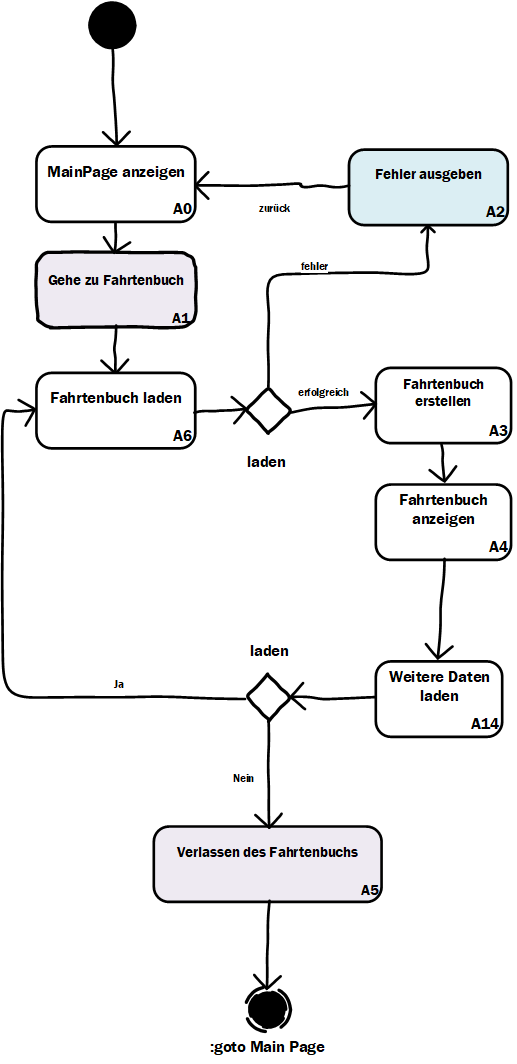
\includegraphics[width=10cm]{figures/Ablaufdiagramm_Fahrtenbuch_LD_APP.png}
	\caption{Ablaufdiagramm Fahrtenbuch}
	\label{fig:Ablaufdiagramm1}
\end{figure}

\begin{figure}[H]
	\centering
	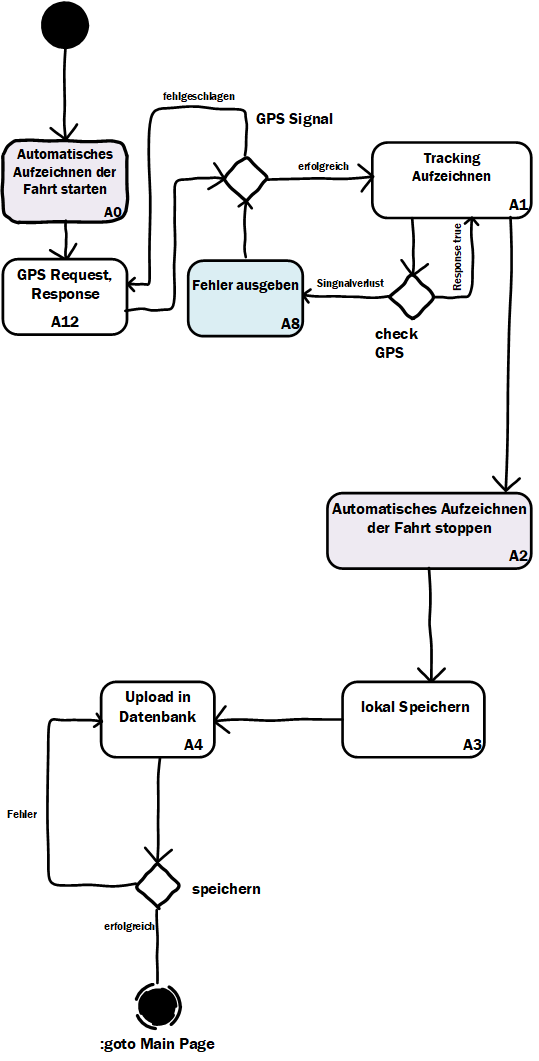
\includegraphics[width=11cm]{figures/Ablaufdiagramm_Tracking_LD_APP.png}
	\caption{Ablaufdiagramm GPS-Tracking}
	\label{fig:Ablaufdiagramm2}
\end{figure}

\newpage
\subsection{User-Interface-Design}
Wir verwendeten Figma für die Mockups und generellen Designs, Frühzeitige Designs sind in Abbildungen \ref{fig:mockup2}, \ref{fig:mockup1} und \ref{fig:mockup3} zu sehen. Sie zeigen die Erstanmeldung, und die Fahrt-hinzufügen Maske in einem Dark und Light Theme.

\begin{figure}[H]
	\centering
	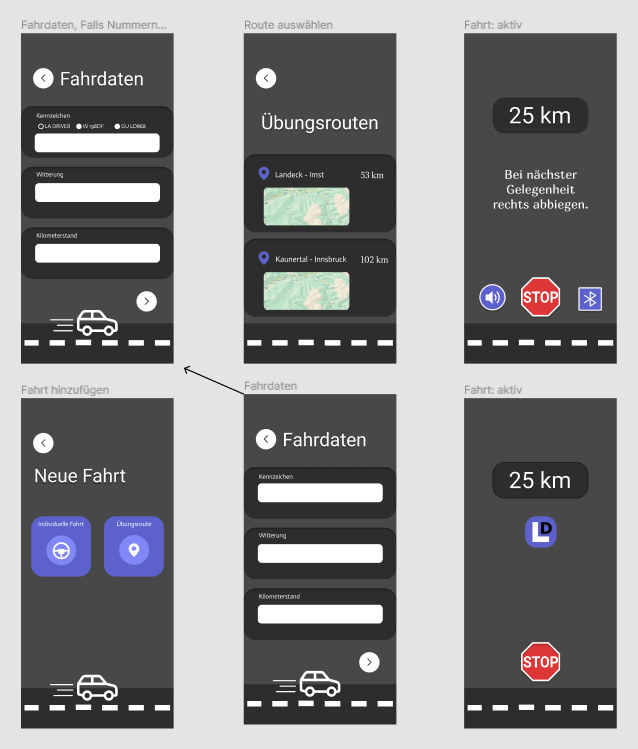
\includegraphics[width=15cm]{figures/mockup2.png}
	\caption{Fahrt hinzufügen im Dark Theme}
	\label{fig:mockup2}
\end{figure}

\begin{figure}[H]
	\centering
	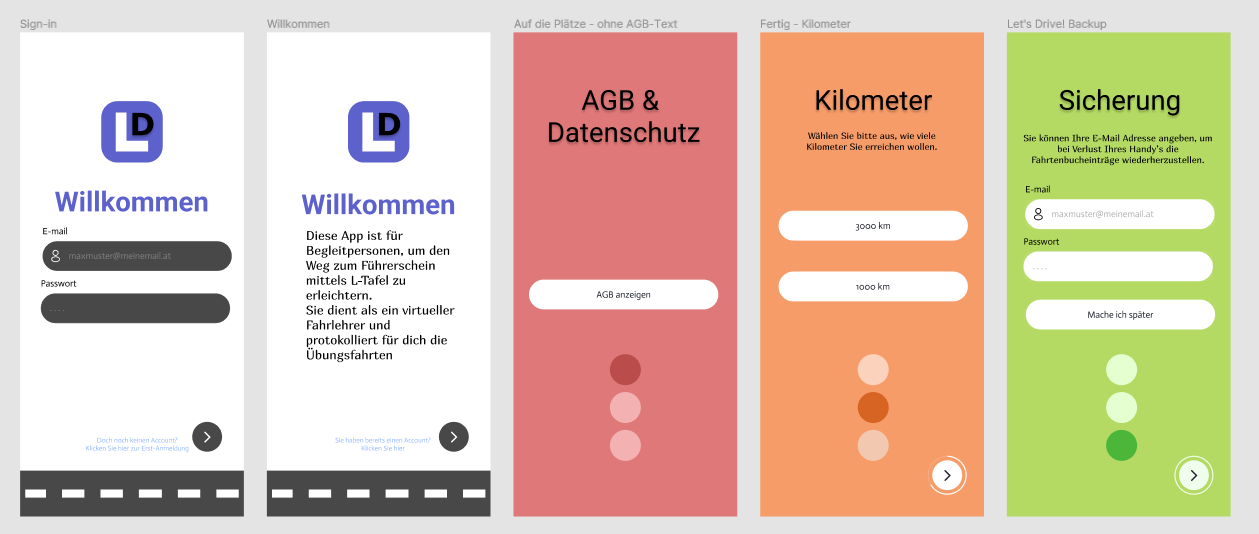
\includegraphics[width=15cm]{figures/mockup1.png}
	\caption{Anfangpages Mockup}
	\label{fig:mockup1}
\end{figure}

\begin{figure}[H]
	\centering
	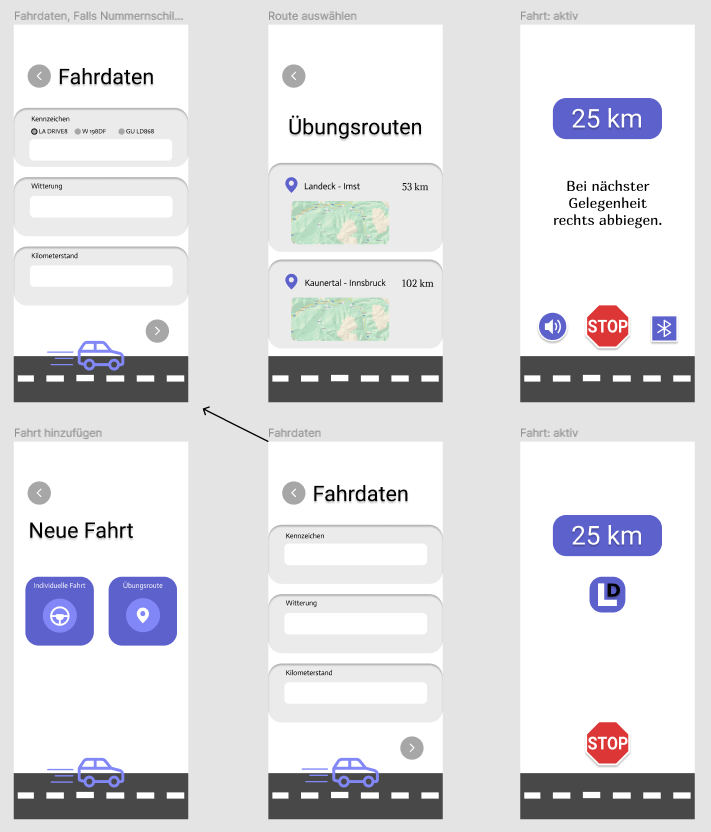
\includegraphics[width=15cm]{figures/mockup3.png}
	\caption{Fahrt hinzufügen im Light Theme}
	\label{fig:mockup3}
\end{figure}

\section{Planung}
Die Planung eines Software-Produktes ist ein essentieller Teil des gesamten Projektes. Vor allem bei einer App wie dieser müssen viele Elemente vorher bestimmt werden. Trotz der agilen Vorgehensweise ist es dennoch wichtig einen allgemeinen Überblick über alle Ziele, Elemente und Anforderungen zu behalten. Dafür sorgen die folgenden Unterpunkte in denen der Projektstrukturplan, die Meilensteine und der Ablaufplan gezeigt werden. Es wird auch ein Kanban-Board verwendet, bei dem der Status einzelner Features eingesehen werden kann.

\subsection{Projektstrukturplan}
Der Projektstrukturplan (in Abbildung \ref{fig:projektstrukturplan}) unterteilt das Projekt in die einzelnen Projektphasen und grobe Arbeitspakete oder Tasks, die diesen Phasen untergeordnet sind. Eine zeitliche Einteilung erfolgt hier nicht. Der Strukturplan wird vor Beginn des Projekts gemacht, um Inhalte zu erfassen.

\begin{figure}[H]
	\centering
	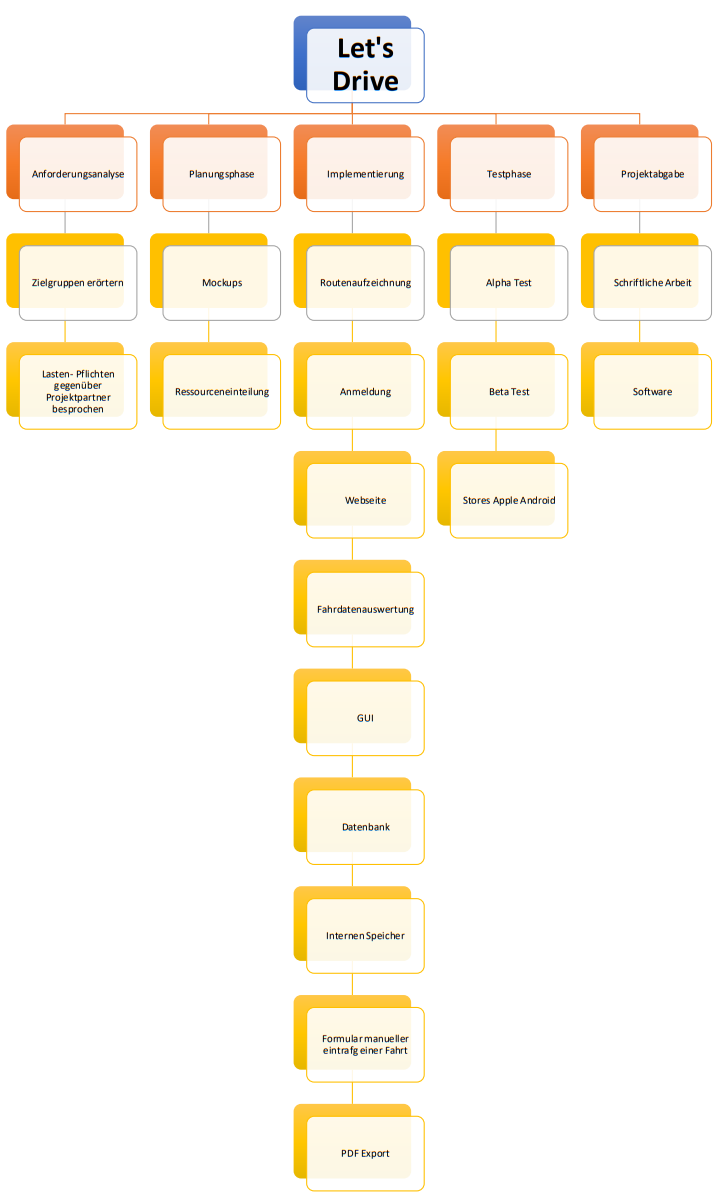
\includegraphics[width=\textwidth,height=\textheight,keepaspectratio]{figures/ProjektStrukturPlan.png}
	\caption{Projektstrukturplan}
	\label{fig:projektstrukturplan}
\end{figure}

\subsection{Meilensteine}
Die Meilensteine, welche mittels flags in Abbildung \ref{fig:ablaufplan} dargestellt werden, markieren entscheidende Etappen im Projektverlauf, wessen Erfüllung den Fortschritt und Erfolg des Projektes quantifizierbar macht. Das Erreichen eines Meilensteins ist immer ein Abschluss einer großen Teilaufgabe eines Projektes. Untergeordnet zu den Meilensteinen sind Sprints, Roadmaps oder Features die das Erreichen der Meilensteine ermöglichen. Übergeordnet sind Epics, welche wiederum viele Meilensteine beinhalten - ein Beispiel wäre das Deployment des ersten Releases.


\subsection{Ablaufplanung}
Der Ablaufplan - bei Azure-Devops heißt dieser Delivery Plan - skizziert den zeitlichen Verlauf des Projektes und gibt Aufschluss darüber, wann welche Teile des Produktes fertiggestellt werden. Mit Azure-Devops lassen sich zeitliche Kapazitäten, der Status, der zuständige Entwickler, Userstories und Tasks darstellen. Azure-Devops ist hier sehr vielseitig. In diesem Ablaufplan, bei der Abbildung \ref{fig:ablaufplan} sind nur die zugeordneten Features zeitlich eingeblendet. Im Kanban - zu sehen in Abbildung \ref{fig:kanban} - werden diese Daten auch dargestellt.

\begin{figure}[H]
	\centering
	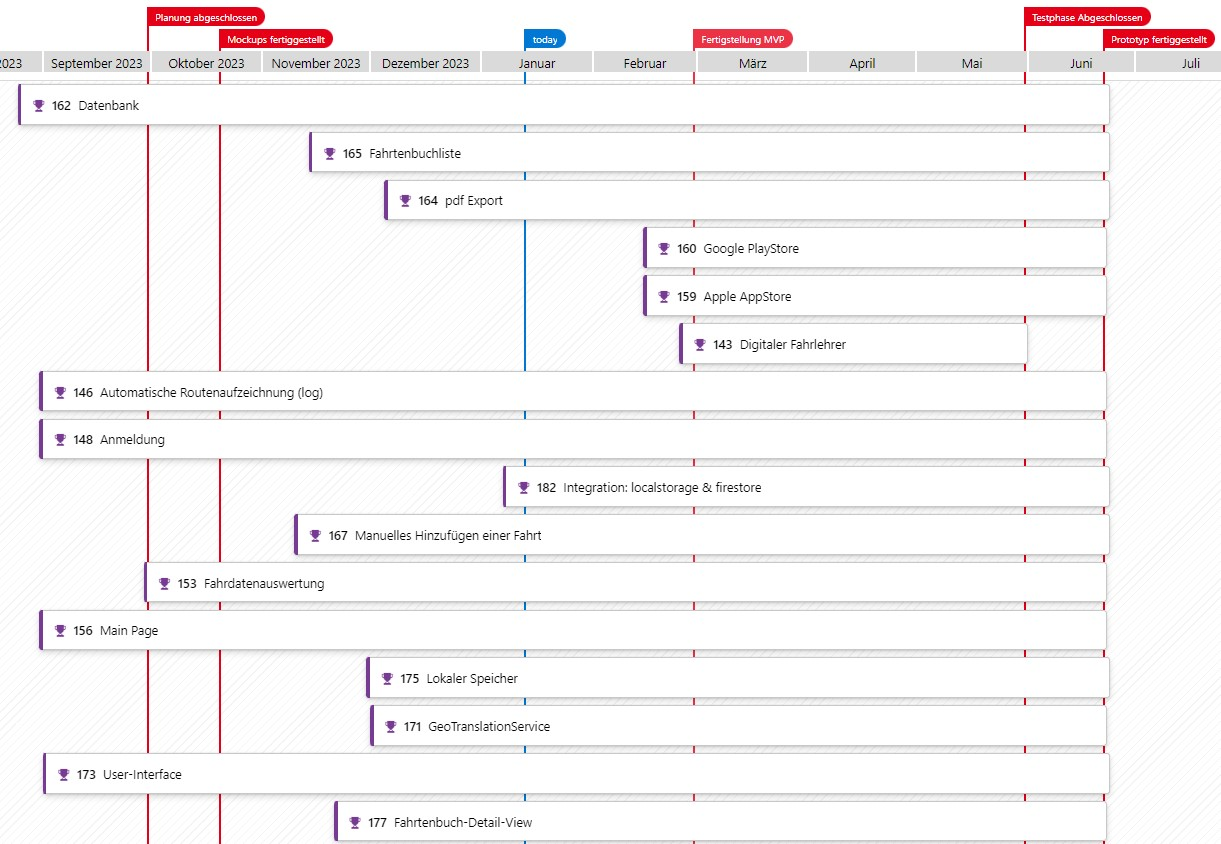
\includegraphics[width=\textwidth,height=\textheight,keepaspectratio]{figures/deliveryplan.jpg}
	\caption{Ablaufplan Let's Drive}
	\label{fig:ablaufplan}
\end{figure}

\begin{figure}[H]
	\centering
	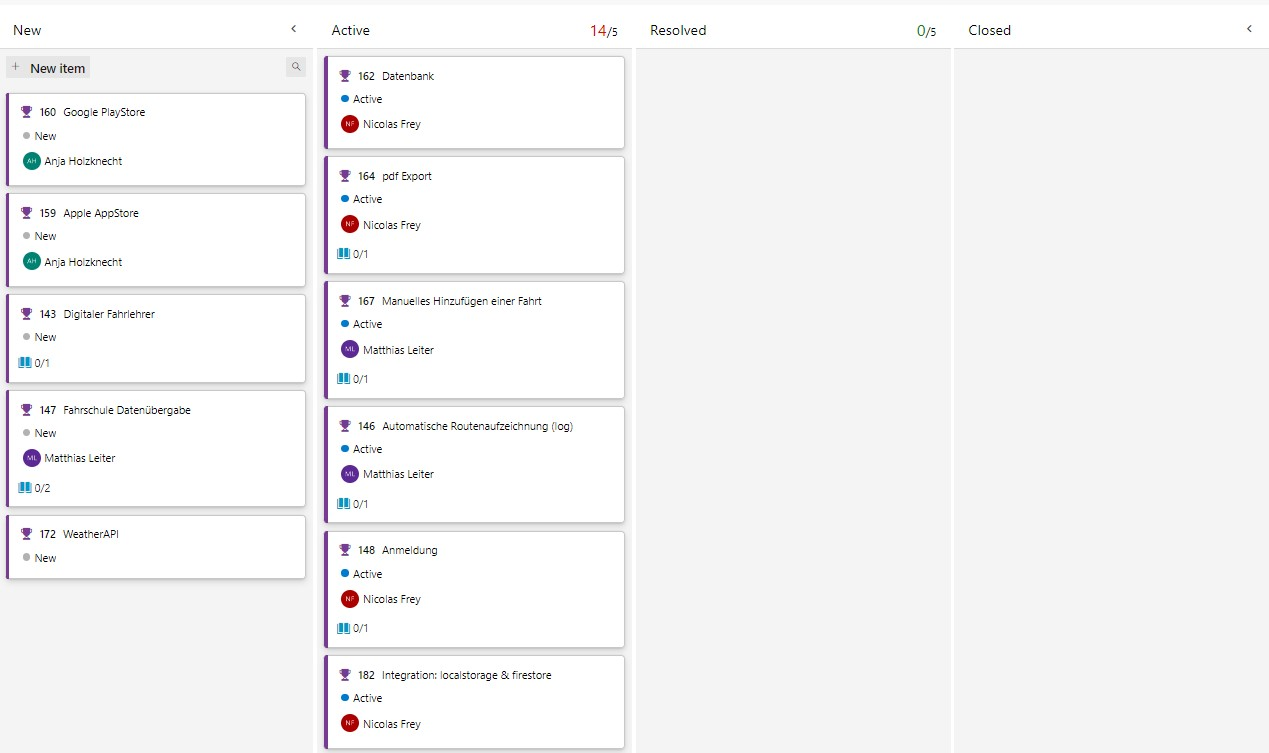
\includegraphics[width=\textwidth,height=\textheight,keepaspectratio]{figures/kanban.jpg}
	\caption{Kanban Let's Drive}
	\label{fig:kanban}
\end{figure}

 

\subsection{Abnahmekriterien}
// TODO
Die Abnahmekriterien definieren die Standards und Voraussetzungen, die erfüllt sein müssen, damit ein Produkt oder eine Phase als abgeschlossen betrachtet werden kann.

\subsection{Pläne zur Evaluierung}
// TODO
Evaluationspläne werden erstellt, um die Leistung des Projektes oder seiner Bestandteile zu bewerten und gegebenenfalls Anpassungen vorzunehmen.

\subsection{Ergänzungen und zu klärende Punkte}
// TODO
In diesem Abschnitt werden zusätzliche Aspekte und offene Fragen festgehalten, die während des Projektverlaufs aufkommen und geklärt werden müssen.

\chapter{Vorstellung des Produktes}
Vorstellung des fertigen Produktes anhand von Screenshots, Bildern, Erklärungen.

\chapter{Eingesetzte Technologien}
Die Entscheidung das Cross Plattform Framework .NET Maui zu verwenden haben wir auf Wunsch des Projektpartners getroffen. Dieses Framework ist von Microsoft und die Programmiersprache ist C\# bzw. XAML für das User Interface. Alternativen wie Google-Flutter gibt es viele, wobei wir auch über eine native Programmierung gesprochen haben.

\section{Architektur}

Das Framework .NET Maui unterstützt die Plattformen Windows, Apple iOS, iPadOS, macOS, Google Android und weitere. Je nach Zielplattform auf die man den Buildvorgang startet unterscheidet sich die Kompilierung. Im Wesentlichen wird der App Code in C\# geschrieben und ist für alle Zielplattformen gültig (oberste Schicht in Abb. \ref{fig:MauiArchitektur}). Die .NET Zugriffe in Abb. \ref{fig:MauiArchitektur} sind in der Programmierung Application Interfaces kurz API´s, welche beispielsweise plattformunabhängige Hardwarezugriffe sein können. Ein anderes Beispiel dafür ist das Erstellen eines nativen Userinterfaces aus dem XAML Progammcode auf eine Zielplattform wo sich Android und iOS unterscheiden. Dieser Zugriff kann auch spezifisch auf eine Zielplattform geschehen also quasi konsistent. So funktioniert in dieser App der implementierte Foreground-Service zum Tracken, welcher nach schließen der App weiterläuft, nur für das Android Betribssystem und ist für iOS anders implementiert. Die zugrundeliegende Runtime für Maui ist die Monoruntime und nicht die bei reinen Windows Apps verwendete Common Language Runtime. Die  Monoruntime stellt z.B. einen Just in Time Compiler kurz JIT und einen Ahead of Time Compiler kurz AOT zur Verfügung. Dabei ist ein JIT kein Interpreter da dieser bereits umgewandelten Code Cachen kann und Codeabschnitte anstelle von Codezeilen in Maschinencode übersetzt. Der AOT übersetzt immer alles in Maschinencode was zum Beispiel bei iOS notwendig ist.

\begin{figure}[H]
	\centering
	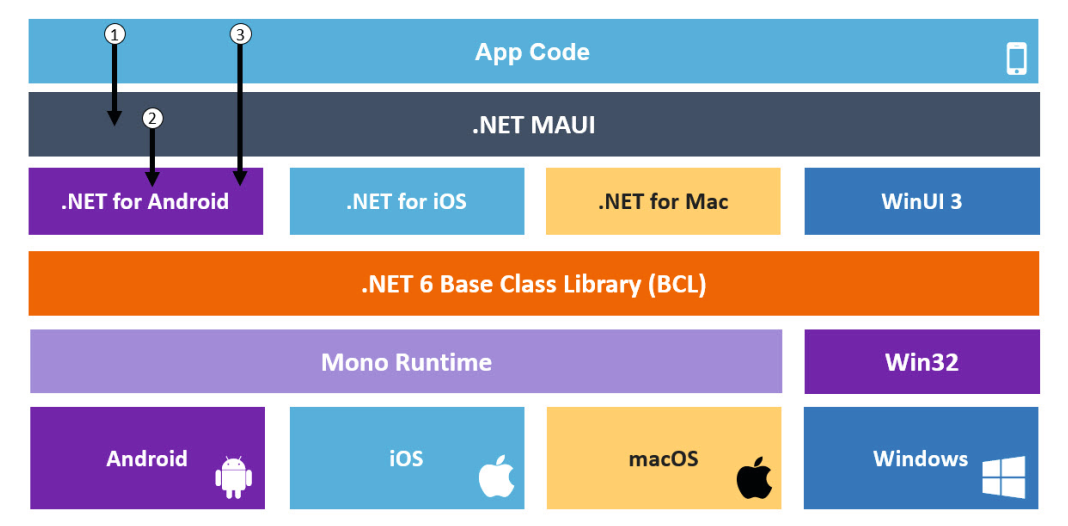
\includegraphics[width=\textwidth,height=\textheight,keepaspectratio]{figures/MauiArchitektur.png}
	\caption{Maui App Architektur bzw. Schichtenmodell}
	\label{fig:MauiArchitektur}
\end{figure}

\subsection{Android Architektur}
Bei Android Smartphones wird die Monoruntime (Mono) parallel zur Android Runtime (ART) ausgeführt. Dabei wird der C\# Code in die Intermediate Language übersetzt der durch die Monoruntime zur Ausführungszeit Just In Time in Maschinencode übersetzt wird (Abb. \ref{fig:AndroidArchitektur}). Die Möglichkeit dies wie in Abb. \ref{fig:AppleÜbersetzung} also Ahead of Time zu kompilieren gibt es auch bei Android. Die vorhin angesprochene Intermediate Language (IL) kann man sich wie den Bytecode oder Zwischencode in Java vorstellen. Die IL ist allgemein für mehrere Microsoft Programmiersprachen wie VB.NET oder F\# gleich. 

\begin{figure}[H]
	\centering
	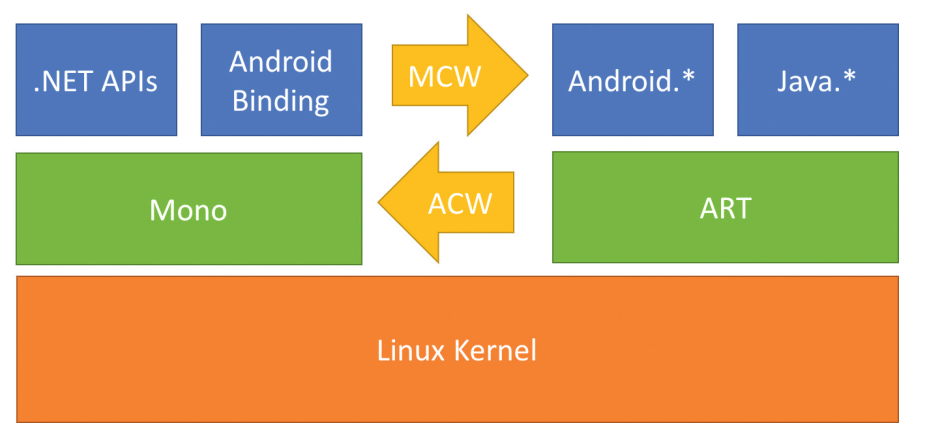
\includegraphics[width=\textwidth,height=\textheight,keepaspectratio]{figures/AndroidArchitektur.png}
	\caption{Android Architektur bzw. Schichtenmodell}
	\label{fig:AndroidArchitektur}
\end{figure}

\subsection{.NET Maui unter Apple Betriebssystemen}
Bei Apple im speziellen bei dieser App dem Betriebssystem iOS muss immer alles in den native Maschinencode kompiliert werden, da Apple das dynamische kompilieren nicht unterstützt. (Abb. \ref{fig:AppleÜbersetzung})

\begin{figure}[H]
	\centering
	\includegraphics[width=\textwidth,height=\textheight,keepaspectratio]{figures/AppleÜbersetzung.png}
	\caption{Aplle Ahead of Time Kompilierung}
	\label{fig:AppleÜbersetzung}
\end{figure}


\chapter{Systementwurf}


\subsection{C4 - Modell}

Beschreibung der Architektur der Software unter Verwendung des C4 Modells: \url{https://c4model.com/}.

Darstellung und Beschreibung der Systemarchitektur.

\begin{itemize}
	\item  statische Zerlegung des Systems in seine physischen Bestandteile (Komponenten, Komponentendiagramm)
	\item (textuelle) Beschreibung des dynamischen Zusammenwirkens aller Komponenten
	\item (textuelle) Beschreibung der Strategie für die Architektur, d. h. wie die Architektur in Statik und Dynamik funktionieren soll.
	\item Verwendung von Referenzarchitekturen bzw. Architekturmustern (als Schablonen, z.B. MVC. Plugin, Pipes and Filters)
	      \begin{itemize}
		      \item MVC
		      \item Schichten
		      \item Pipes
		      \item Request Broker
		      \item Service-Oriented
	      \end{itemize}
\end{itemize}

\subsection{Benutzerschnittstellen}
\begin{itemize}
	\item Design des UIs
	\item Dialoge, Dialogsteuerung, Ergonomie, Gestaltung, Eingabeüberprüfungen
\end{itemize}

\subsection{Datenhaltunskonzept}
\begin{itemize}
	\item Design der Datenbank (ER-Modell)
	\item Design des Zugriffs auf diese Daten (Datenhaltungskonzept)
	\item Caching, Transaktionen
\end{itemize}

\subsection{Konzept für Ausnahmebehandlung}
\begin{itemize}
	\item Systemweite Festlegung, wie mit Exceptions umgegangen wird
	\item Exceptions sind primär aus den Bereichen UI, Persistenz, Workflow-Management
\end{itemize}

\subsection{Sicherheitskonzept}
Beschreibung aller sicherheitsrelevanten Designentscheidungen

\begin{itemize}
	\item Design der Security-Elemente
	\item Design von Safety-Elementen (Fehlertoleranz, Verfügbarkeit etc.)
\end{itemize}

\subsection{Design der Testumgebung}
\begin{itemize}
	\item wie wird getestet (Unit-Testing, Integrationstesting, Systemtests, Akzeptanztests)
	\item Testumgebung, Testprozess, Teststrategie, Testmethoden, Testfälle
\end{itemize}


\subsection{Desing der Ausführungsumgebung}
\begin{itemize}
	\item Deployment (DevOps)
	\item Betrieb (besonders Hoch- und Hertunerfahren der Anwendung)
\end{itemize}

\section{Detailentwurf}

Design jedes einzelnen USE-Cases

\begin{itemize}
	\item Design-Klassendiagramme vom Domain-Klassendiagramm ableiten (incl. detaillierter Darstellung und Verwendung von Vererbungshierarchichen, abstrakten Klassen, Interfaces)
	\item Sequenzdiagramme vom System-Sequenz-Diagramm ableiten
	\item Aktivitätsdiagramme
	\item Detaillierte Zustandsdiagramme für wichtige Klassen
\end{itemize}

Verwendung von CRC-Cards (Class, Responsibilities, Collaboration) für die Klassen
\begin{itemize}
	\item um Verantwortlichkeiten und Zusammenarbeit zwischen Klassen zu definieren und
	\item um auf den Entwurf der Geschäftslogik zu fokussieren
\end{itemize}

Design-Klassen für jeden einzelnen USE-Case können z.B. sein:

\begin{itemize}
	\item UI-Klassen
	\item Data-Access-Klassen
	\item Entity-Klassen (Domain-Klassen)
	\item Controller-Klassen
	\item Business-Logik-Klassen
	\item View-Klassen
\end{itemize}

Optimierung des Entwurfs (Modularisierung, Erweiterbarkeit, Lesbarkeit):

\begin{itemize}
	\item Kopplung optimieren
	\item Kohäsion optimieren
	\item SOLID
	\item Entwurfsmuster einsetzen
\end{itemize}

\chapter{Implementierung}
Detaillierte Beschreibung der Implementierung aller Teilkomponenten der Software entlang der zentralsten Use-Cases:

\begin{itemize}
	\item GUI-Implementierung
	\item Controllerlogik
	\item Geschäftslogik
	\item Datenbankzugriffe
\end{itemize}

Detaillierte Beschreibung der Teststrategie (Testdriven Development):

\begin{itemize}
	\item UNIT-Tests (Funktional)
	\item Integrationstests
\end{itemize}

Zu Codesequenzen:
\begin{itemize}
	\item kurze Codesequenzen direkt im Text (mit Zeilnnummern auf die man in der Beschreibung verweisen kann)
	\item lange Codesequenzen in den Anhang (mit Zeilennummer) und darauf verweisen
\end{itemize}

\chapter{Deployment}
\begin{itemize}
	\item Umsetzung der Ausführungsumgebung
	\item Deployment
	\item DevOps-Thema
\end{itemize}

\chapter{Tests}

\section{Systemtests}
Systemtests aller implementierten Funktionalitäten lt. Pflichtenheft
\begin{itemize}
	\item Beschreibung der Teststrategie
	\item Testfall 1
	\item Testfall 2
	\item Tesfall 3
	\item …
\end{itemize}

\section{Akzeptanztests}

\chapter{Projektevaluation}
siehe Projektmanagement-Unterricht

\chapter{Benutzerhandbuch}
falls im Projekt gefordert

\chapter{Betriebswirtschaftlicher Kontext}
BW-Teil

\chapter{Zusammenfassung}
Mit der Projektumfeldanalyse wurden alle Stakeholder erfasst, die bei einer praktisch ausgelegten App für L17 Fahrschüler:innen als relevant erschienen. Die Positionen der einzelnen Interessensgruppen wurden analysiert und grafisch dargestellt. Weiters wurde ein Maßnahmenkatalog erstellt, um mögliche Methoden zu identifizieren, die das Projektumfeld verbessern sollen. Da dieses Projekt mit der Diplomarbeit am IT-Kolleg zusammenhängt ist der Termin mit Ende Juni für ein Minimum Viable Produkt festgelegt. Dieser Termin ist aber sehr realistisch. Die Anforderungen an diese App sind für eine Smartphone App umfangreich und erfordern eine genaue Auswertung und Prüfung in der Testphase. Dieses Produkt bietet dem/der Fahrschüler:in eine Erleichterung bei der Protokollierung und laufend Feedback über den praktischen Fortschritt dem/der Schüler:in.
